\documentclass[12pt]{article}

%%%%%%%%%%%%%%%%%%%%%%%%%%%%
%%%%%%%%%%%%%%%%%%%%%%%%%%%%
% Load in packages
\usepackage{amsmath}
\usepackage{amssymb}
\usepackage{hyperref}
\usepackage{graphicx}
\usepackage[top=1in, bottom=1in, left=1in, right=1in]{geometry}

%%%%%%%%%%%%%%%%%%%%%%%%%%%%
%%%%%%%%%%%%%%%%%%%%%%%%%%%%

\begin{document}

\begin{center}
\Large Chapter 6 Practice Problems Solutions

\medskip

\normalsize Elements of Microeconomics

\medskip

\small Discussion section 4
\end{center}

\medskip

\section*{Question 1}
This question will consider a market for coffee, which is depicted in figure \ref{fig:coffee_eq}.

\begin{figure}[h]
    \centering
    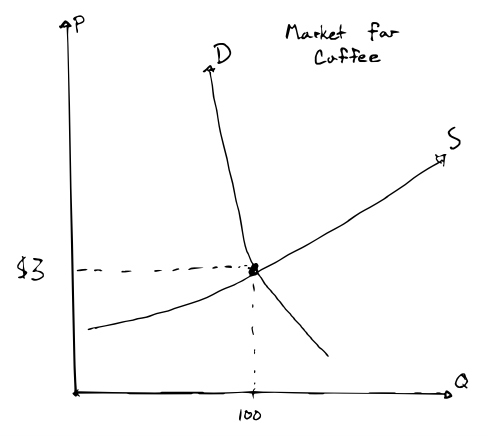
\includegraphics[width=.6\textwidth]{coffee_eq.png}
    \caption{Market for coffee}
    \label{fig:coffee_eq}
\end{figure}

\subsection*{Part A}
Consider two price ceilings:
    \begin{itemize}
        \item At \$2.5
        \item At \$3.5
    \end{itemize}

    \vspace{5mm}

    In both of these cases depict graphically the new market outcome, and answer:
    \begin{enumerate}
        \item What happens to the new quantity demanded and supplied?
        \item Does the policy cause a shortage or a surplus?
        \item Is the policy binding? Why or why not?
    \end{enumerate}

\subsection*{Part B}
Repeat the same exercise but for a price \textit{floor} at \$2.5 and \$3.5.

\section*{Question 2}

\subsection*{Part A}
Consider the market for Orioles tickets:
\begin{enumerate}
    \item Which side is elastic?
    \item Which side is inelastic?
    \item What might happen in the long run?
\end{enumerate}

Draw two graphs illustrating your answers, one in the short-run and one in the long-run.

\subsection*{Part B}
Now suppose Baltimore City imposes a \textit{binding} price floor on tickets:
    \begin{enumerate}
        \item What is the impact in the short-run?
        \item What is the impact in the long-run?
        \item Is the impact larger in the short-run or long-run?
    \end{enumerate}

\section*{Question 3}
Let's consider the coffee market from Question 1 again. Instead of price controls (rare in advanced economies), consider a tax of \$0.5 per cup applied to suppliers:

\begin{enumerate}
    \item Does this shift supply or demand curves?
    \item What will happen to equilibrium price and quantity?
    \item What portion falls on consumers and what falls on suppliers?
\end{enumerate}

Draw a graph to illustrate the intuition behind your answers (I am not looking for specific numbers since you are not provided with functions). Make sure to draw the tax wedge, labeling the portion falling on consumers and on suppliers.

\subsection*{Part B}
Draw two graphs to illustrate the same tax when demand is perfectly inelastic, and when supply is perfectly inelastic. Explain the intuition for who bears the tax burden and why.

\subsection*{Part C}

Repeat this exercise, but considering the tax as levied on consumers rather than producers. Does the tax burden depend on how the tax is imposed?

\end{document}